% qPCRtools — Bioinformatics (Oxford) Application Note
%
% NOTE: 投稿前将 \documentclass 替换为 Bioinformatics 官方 Application Note
%       模板 (cls)，并按官方要求调整 bst 与排版参数。当前用 article 骨架，
%       便于在 Overleaf 上编辑预览。
%
% 投稿要点（2026-10-15 按官方 Application Note 说明对齐）：
%  1) 官方原文（Bioinformatics, Instructions to Authors，由用户 2026-10-15 提供）：
%     "Application Notes — Up to 4 pages; this is approx. 2,600 words or 2,000 words plus one figure"。
%     本稿按更严的"2,000 词 + 1 图"档执行：正文 1,777 词（摘要 231），主文只留
%     1 图（界面截图）+ 1 表（工具功能对比）；标准曲线/表达量图、等价性散点与等价性汇总表
%     移入 supplementary.tex（Figure S1–S2、Table S1）。
%  2) 官方另三条硬要求已满足：Availability and Implementation 在正文写明（含"至少两年可用"承诺）；
%     补充材料在摘要中提及；题目含软件名 qPCRtools。
%  3) 投稿时需在系统内提名一位 Associate Editor。
%  3) 作者与单位（2026-10-13 用户确认）：Xiang Li（第一作者 + 通讯）、Huichuan Huang（共同通讯）；
%     两人单位均为 1、2；Xiang Li 现地址为 Yazhouwan National Laboratory（present address）。
\documentclass[11pt]{article}

\usepackage[utf8]{inputenc}
\usepackage{graphicx}
% hidelinks：链接保持可点击，但不画彩色边框、不变色（hyperref 默认会给引用画绿框、
% 给 URL 画品红/青框，投稿时应当关掉——2026-10-13 用户指出参考文献处出现绿框）
\usepackage[hidelinks]{hyperref}
\usepackage{booktabs}
\usepackage{amsmath}

\title{qPCRtools: a cross-platform C++ desktop application for qPCR data
analysis with validated equivalence to its R implementation}

\author{%
\parbox{\textwidth}{\centering\sloppy
Xiang Li\textsuperscript{1,2,*} \quad Huichuan Huang\textsuperscript{1,2,*}\\[6pt]
\textsuperscript{1}~State Key Laboratory for Conservation and Utilization of Bio-Resources in Yunnan,
Yunnan Agricultural University, Kunming, China\\
\textsuperscript{2}~Key Laboratory for Agro-Biodiversity and Pest Control of Ministry of Education,
Yunnan Agricultural University, Kunming, China\\[6pt]
\textsuperscript{*}~Corresponding authors: \texttt{lixiang117423@gmail.com} (X.L.),
\texttt{absklhhc@gmail.com} (H.H.)\\
Present address (X.L.): Yazhouwan National Laboratory, Sanya, Hainan, China
}%
}

\date{}  % Application Note 通常不显示日期

\begin{document}
\maketitle

\begin{abstract}
Quantitative real-time PCR (qPCR) is a standard technique for measuring gene
expression, yet turning instrument-exported $C_q$ values into
publication-ready results requires several non-trivial steps: estimating
amplification efficiency, choosing a quantification method, testing groups
statistically, and preparing figures. Established tools for this chain are
predominantly programming-based---including our own R package
\textit{qPCRtools}---and remain out of reach for students and wet-lab
researchers without programming experience, whereas instrument software, free
stand-alone programs and web applications each cover only part of the
workflow or tie the analysis to one platform. We present \textit{qPCRtools},
a cross-platform desktop application written in C++17 with Qt6 that exposes
the analytical core of the R package through a point-and-click interface and
ships as a single executable requiring no R, Python or other runtime. It
implements standard-curve construction and efficiency estimation, the
$\Delta C_t$, $\Delta\Delta C_t$ and efficiency-based (RqPCR) quantification
methods, group comparison by Welch $t$-test, Wilcoxon rank-sum test or
one-way ANOVA with Tukey HSD letters, quality-control warnings,
in-interface figures, and a plain-text record of the inputs and parameters of
each analysis. On identical inputs the C++ implementation agrees with the R
package to floating-point precision for every shared method; preparing the
port also revealed and corrected several defects in result aggregation, each
covered by a regression test. Supplementary figures and tables give the full
analysis output and the equivalence comparison, and the availability and
implementation statement appears at the end of the article.
\end{abstract}

\section{Introduction}

Quantitative real-time PCR (qPCR) is among the most widely used techniques
in molecular biology for quantifying nucleic acids and measuring gene
expression \cite{bustin2009miqe}. Current reporting guidance is provided by
MIQE~2.0 \cite{bustin2025miqe2}. A sound analysis involves several
interdependent steps: estimating primer amplification efficiency, choosing a
quantification strategy, testing groups statistically, and preparing figures
\cite{bustin2010miqe}. When target and reference efficiencies are comparable,
the $2^{-\Delta\Delta C_T}$ method \cite{livak2001analysis} is convenient;
when they differ, an efficiency-corrected or standard-curve-based approach is
required \cite{pfaffl2001new}. These choices, combined with the need for
rigorous statistics, make qPCR analysis demanding for many laboratory
researchers.

{\sloppy A range of tools cover different parts of this workflow
(Table~\ref{tab:tools}). Scripting-based implementations---our own
\textit{qPCRtools} \cite{li2022qpcrtools} and \textit{pcr}
\cite{ahmed2018pcr}---implement the calculation chain transparently but
require programming skill and a configured environment. Software distributed
with real-time instruments (for example QuantStudio Design \& Analysis and
CFX Maestro) offers a graphical workflow but is tied to that instrument.
Free stand-alone programs cover single steps: REST \cite{pfaffl2002rest}
computes efficiency-based relative expression for two-group comparisons with
a randomisation test, LinRegPCR
\cite{ramakers2003linregpcr,ruijter2009linregpcr} estimates baseline and
efficiency from raw fluorescence, and qBase \cite{hellemans2007qbase}
implements relative quantification with the geNorm stability measure
\cite{vandesompele2002accurate}. Free web applications---SATQPCR
\cite{rancurel2019satqpcr}, DAG Expression \cite{ballester2013dag} and
Auto-qPCR \cite{maussion2021autoqpcr}---integrate several steps but require
uploading the data to a remote server or deploying the web stack locally. The
gap is therefore not a missing algorithm but a missing delivery mode:
\emph{auditable numerical implementation} combined with a \emph{native,
cross-platform, zero-dependency} graphical workflow.
\par}

\begin{table}[h]
\centering
\footnotesize
\setlength{\tabcolsep}{2pt}
\caption{Delivery mode and functionality of representative qPCR analysis
tools. ``Free for non-commercial use'' means no purchase is required for
academic users; software distributed with an instrument is marked as not
free. ``Reference-gene stability'' denotes computational selection or ranking
of reference genes, not merely normalisation to a chosen reference gene.
$\bullet$~provided, $\circ$~not provided, $\circ$/$\bullet$~partial or
version-dependent (statistics were added in the later qBase+ release; vendor
software differs between instruments and versions). Compiled from the cited
papers, the vendors' documentation and the survey of Pabinger \textit{et al.}
\cite{pabinger2014survey}. \textsuperscript{a}~\textit{qPCRtools}
\cite{li2022qpcrtools}, \textit{pcr} \cite{ahmed2018pcr}, qpcR
\cite{ritz2008qpcr}, NormqPCR \cite{perkins2012normqpcr}, and the archived
Bioconductor package EasyqpcR \cite{lepape2017easyqpcr}.
\textsuperscript{b}~QuantStudio Design \& Analysis, CFX Maestro.
\textsuperscript{c}~SATQPCR \cite{rancurel2019satqpcr}, DAG Expression
\cite{ballester2013dag}, Auto-qPCR \cite{maussion2021autoqpcr}.}
\label{tab:tools}
\begin{tabular}{lcccccc}
\toprule
Tool & Free & No coding & Offline & Efficiency & Statistics & Ref.-gene stability \\
\midrule
R packages\textsuperscript{a} & $\bullet$ & $\circ$ & $\bullet$ & $\bullet$ & $\circ$/$\bullet$ & $\bullet$ \\
This application & $\bullet$ & $\bullet$ & $\bullet$ & $\bullet$ & $\bullet$ & $\bullet$ \\
REST & $\bullet$ & $\bullet$ & $\bullet$ & $\bullet$ & $\bullet$ & $\circ$ \\
LinRegPCR & $\bullet$ & $\bullet$ & $\bullet$ & $\bullet$ & $\circ$ & $\circ$ \\
qBase & $\bullet$ & $\bullet$ & $\bullet$ & $\bullet$ & $\circ$ & $\bullet$ \\
qBase+ & $\circ$ & $\bullet$ & $\bullet$ & $\bullet$ & $\bullet$ & $\bullet$ \\
Instrument software\textsuperscript{b} & $\circ$ & $\bullet$ & $\bullet$ & $\bullet$ & $\circ$/$\bullet$ & $\circ$ \\
Web apps\textsuperscript{c} & $\bullet$ & $\bullet$ & $\circ$ & $\bullet$ & $\bullet$ & $\bullet$ \\
\bottomrule
\end{tabular}
\end{table}

\subsection*{Statement of need}

The programming requirement is not a marginal obstacle. In our own teaching
and collaborative work, the users who most need a defensible qPCR analysis
are frequently those least able to install an R environment and write the
few lines of code the analysis requires: newly enrolled students, visiting
researchers, and wet-lab staff whose projects run for a single season. They
fall back either on manual spreadsheet calculations---difficult to audit and
easy to get wrong---or on whichever instrument software happens to be
installed. Our R package \cite{li2022qpcrtools} provides the algorithms, but
its use is bounded by the R environment itself.

As a pragmatic test of the workflow, we re-analysed the two real example
plates distributed with the 2022 \textit{qPCRtools} paper: one four-fold
dilution series and one separate treatment plate with four biological
replicates. Both analyses were completed through the graphical interface and
exported with a parameter record, without a spreadsheet or custom script
(Supplementary Table~S3). This is a reproducible published-data re-analysis,
not a controlled human-factors trial.

We therefore reimplemented the analytical core as a native desktop
application that implements the same three quantification methods while
removing every prerequisite except a double-click. \textit{qPCRtools} makes
three contributions: (i)~a C++/Qt architecture in which a tested core
algorithm library is decoupled from a web-based user interface; (ii)~a
reproducible validation against an independent base-R reference across all
quantification methods; and
(iii)~statistical and functional extensions beyond the R version
(non-parametric tests, effect sizes, outlier removal, quality-control
warnings, automatic reference-gene selection). Preparing the port also
revealed defects in result aggregation shared with the R package---the input
of the reference-gene stability measure, replicate handling in the efficiency
method, and the $\Delta\Delta C_t$ calibrator---as well as one specific to the
C++ code (multiple-comparison $P$-values); all were corrected and are covered
by regression tests.

\section{Implementation}

\subsection{Architecture}

{\sloppy\textit{qPCRtools} is written in C++17 and built on Qt6 \cite{qt}. The user
interface is rendered with web technologies---Bootstrap~5.3 for layout and
Apache ECharts \cite{echarts} for figures---inside a
\texttt{QWebEngineView}, and exchanges data with the native backend through
Qt~WebChannel. All numerical computation therefore stays in compiled code
while the presentation layer remains plain HTML, CSS and JavaScript. The
analytical core is a standalone static library, \texttt{qpcr\_core}, that
depends only on Qt~Core (plus optional Eigen and GSL) and is independent of
the GUI, so it is exercised directly by the unit tests and by the
command-line validation driver. Figure~\ref{fig:overview} shows the
interface at the end of a complete analysis.\par}

\begin{figure}[tbp]
\centering
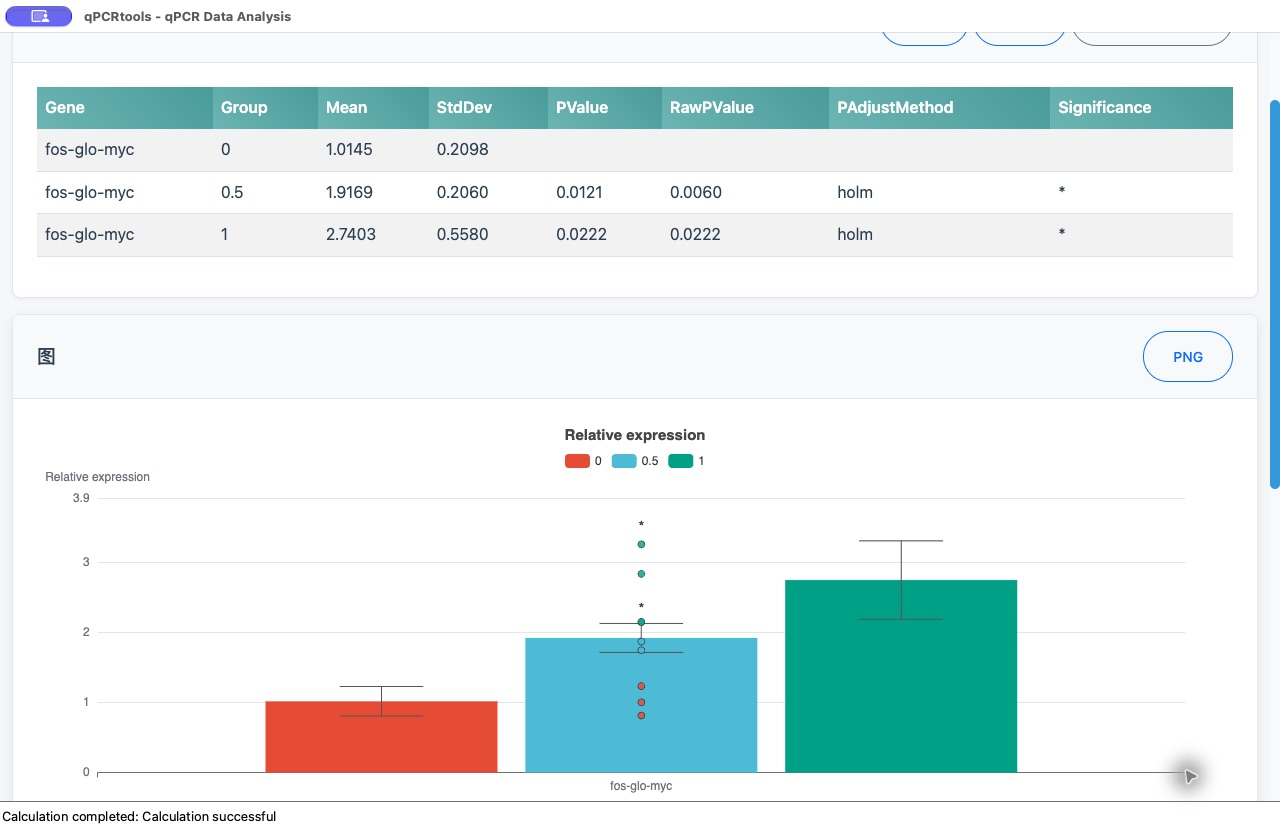
\includegraphics[width=0.85\linewidth]{figures/fig1_results_page_en_v4_20261029.png}
\caption{The \textit{qPCRtools} desktop interface (screen capture of
version~1.3.0). The upper panel is the summary table from the bundled
example---the target gene \textit{fos-glo-myc} normalised to
\textit{Beta Actin},
three dose groups with three biological replicates each---analysed by the
$\Delta\Delta C_t$ method with Welch tests against the control. It reports
the mean, standard deviation, Holm-adjusted and raw $P$ values, adjustment
method and significance symbol. The lower panel redraws the group means with
standard-deviation error bars, individual biological replicates and
Holm-adjusted symbols; the error bars are not repeated as a legend entry.
The interface is bilingual (Chinese/English); the English language is
shown here.}
\label{fig:overview}
\end{figure}

\subsection{Quantification algorithms}

The core reimplements the methods of the R package. Amplification efficiency
is obtained by ordinary least squares of $C_q$ on
$\log_{d}(\text{concentration})$, i.e.\ the number of $d$-fold dilution
steps ($d$ = dilution factor, 4 in the bundled example), yielding slope $s$,
intercept, $R^2$ and a regression $P$-value; efficiency is
\begin{equation}
E = d^{-1/s} - 1,
\end{equation}
with $s$ expressed per $\log_d$ unit (equivalently, per dilution step).
Relative expression is computed by the
$\Delta C_t$ and $\Delta\Delta C_t$ methods \cite{livak2001analysis},
\begin{equation}
\mathrm{RE} = 2^{-\big[(C_{q,\mathrm{target}}-C_{q,\mathrm{ref}})_{\mathrm{treated}}
- \overline{(C_{q,\mathrm{target}}-C_{q,\mathrm{ref}})}_{\mathrm{control}}\big]},
\end{equation}
where the first term is sample-level and the overbar is the mean $\Delta C_t$
across control biological replicates. Relative expression is also computed
by an efficiency-based (RqPCR) method \cite{rancurel2019satqpcr} in which
per-sample quantities are $E^{\,C_{q,\min}-C_q}$, normalized by the geometric
mean of one or more reference genes \cite{pfaffl2001new}. In this method
$C_{q,\min}$ is obtained separately within each biological replicate across
the treatments, so the calculation is a within-block comparison rather than a
general unpaired design. Efficiencies are supplied per gene in the design
table (or estimated by the built-in standard-curve module).

\subsection{Statistical analysis}

{\sloppy Groups are compared on the linear relative-expression scale, which is
the scale on which values are reported and plotted. Because the linear and
$\Delta C_t$ scales can give different $P$ values for the same data, the
$\Delta C_t$-scale comparison is reported as a sensitivity analysis in
Supplementary Table~S2. The core
library implements Welch and Student two-sample $t$-tests, the paired
$t$-test, Wilcoxon rank-sum and signed-rank tests, one-way ANOVA with Tukey
HSD letters, Cohen's $d$, IQR-based outlier removal and automatic
reference-gene selection by geNorm \cite{vandesompele2002accurate}; the
interface exposes the Welch $t$-test, the rank-sum test and ANOVA with Tukey
HSD, while the paired tests are covered by the test suite but not yet offered
in the interface. When several groups are compared with the same control,
Welch and rank-sum $P$ values are adjusted by Holm's method within each gene,
and the unadjusted value is retained in the exported table. ANOVA uses Tukey
HSD. Correction is not applied across genes, which we state as a
limitation.\par}

\subsection{Software engineering and scope}

Results are shown as tables that can be exported as CSV or Excel, with Tukey
letters in the table. The application renders the figures in the interface:
group means with standard-deviation error bars and significance labels, and
the fitted standard curves over the measured dilution series, both exportable
as PNG images. Each analysis can also be exported as a plain-text
\emph{analysis record} listing the input files and their row counts, the
reference gene(s), the control group, the statistical test, the
outlier-removal setting, the software version and a timestamp, so that a
reader can re-run the analysis without inspecting the session. Quality
control is reported as warnings rather than decisions: wells with $C_q$ above
a configurable limit (default 35), samples whose technical replicates differ
by more than a configurable standard deviation (default 0.5~$C_q$), and
primers with efficiency outside 90--110\% are listed on the results page and
repeated in the analysis record, while no data are removed automatically.
MIQE~2.0 requires these quantities to be reported rather than to satisfy fixed
cut-offs \cite{bustin2025miqe2}, so the defaults are meant to be adapted to
the instrument and assay. \textit{qPCRtools} is managed with CMake and ships
with unit tests; the interface is bilingual and reads CSV/TXT input, and Excel
(\texttt{.xlsx}) workbooks when built with the optional OpenXLSX component
(the released binaries read CSV/TXT). It is distributed as a single
self-contained executable for Windows and macOS, requiring no R, Python or
runtime installation. The macOS binary is built for Apple Silicon, requires
macOS~12 or newer, and is ad-hoc signed but not notarized. Linux builds are
supported by the source and build scripts but are not part of the released
binary set. Two R
functions are not yet ported---the standard-curve
slope--intercept quantification (\texttt{CalExpCurve}) and the
reverse-transcription reagent volume calculation (\texttt{CalRTable})---and
are planned for a future release.

\section{Results}

% 纪律：本节所有数值均来自 validation/results/ 的真实输出（R 与 C++ 实跑）。

\subsection{Typical analysis workflow}

{\sloppy We applied the application to the bundled example dataset
(\texttt{examples/cq.csv}, \texttt{examples/design.csv}): the target gene
\textit{fos-glo-myc} against the reference gene \textit{Beta Actin} across
three treatment groups (0, 0.5, 1) with three biological replicates each.
With the $\Delta\Delta C_t$ method and Welch tests against the control,
relative expression rose to 1.92 at dose~0.5 and 2.74 at dose~1, both
significantly different from the control ($p = 0.006$ and $p = 0.022$); as
defined by Livak and Schmittgen the calibrator is the control group, which is
therefore $\approx 1$ (here $1.01 \pm 0.21$). These means, standard
deviations and $p$-values are reproduced without the application or the R
package by \texttt{validation/check\_example\_stats.R}, and the complete
output is shown in Supplementary Figure~S1B. On a four-fold dilution series
of four genes, the standard-curve module recovered slopes of $-2.07$ to
$-2.24$ $C_q$ per dilution step with $R^2 > 0.99$ for three of the four
primers (efficiencies 0.85--0.95; Supplementary Figure~S1A), illustrating the
efficiency estimation that, per MIQE guidance, determines which
quantification method is appropriate. The quality-control panel flagged the
single $C_q = 40$ well of the weakest primer, and the complete
workflow---import, configuration, analysis, export---is performed in the
graphical interface without writing code.\par}

\subsection{Equivalence to the R package}

{\sloppy We ran the C++ implementation and the original R package
\cite{li2022qpcrtools} on identical inputs for every shared
method---$\Delta\Delta C_t$ (\texttt{CalExp2ddCt}), the standard curve
(\texttt{CalCurve}) and the efficiency-based RqPCR method
(\texttt{CalExpRqPCR})---reading the same on-disk files, so any difference
reflects the implementations alone (Supplementary Table~S1 and Figure~S2).
For both expression methods, expression values, standard deviations and
standard errors matched to within floating-point precision (maximum relative
difference $< 4 \times 10^{-15}$). For the standard curve, slope, intercept,
$R^2$ and efficiency agreed to within $2.5 \times 10^{-3}$ relative
difference, the residual being attributable to the R package rounding its
tabulated output to two to four decimals while the underlying $C_q$ inputs
are identical; every point falls on the line $y = x$.\par}

The validation is fully reproducible from the open scripts in
\texttt{validation/} (see Availability). Preparing the port also revealed
defects in result aggregation that the R implementation shared---the input of
the reference-gene stability measure, replicate handling in the efficiency
method and the $\Delta\Delta C_t$ calibrator---as well as one specific to the
C++ code (multiple-comparison $p$-values); each was corrected and is covered
by a regression test.

\section{Availability and implementation}

Implementation: \textit{qPCRtools} is a C++17/Qt6 desktop application built
with CMake ($\geq$~3.20); the core algorithm library requires only Qt~Core and
optionally links Eigen3, GSL and OpenXLSX, while the interface requires
Qt~WebEngine and WebChannel. It is distributed as a single self-contained
executable for Windows and macOS---no R, Python or other runtime, and no
registration, are needed to download or run it---and the source compiles on
Linux.

Availability: version~1.2.0 (the version described here; version~1.1.0 is the
previous release) is freely available under the MIT license at
\url{https://github.com/lixiang117423/qPCRtools_cpp}, with pre-built binaries
in the repository releases. The repository includes documentation, a
unit-test suite, example datasets and a fully reproducible
equivalence-validation package (\texttt{validation/}) comprising the R script,
a C++ command-line driver linked against \texttt{qpcr\_core}, and a comparison
script that regenerates all validation outputs and figures. We will keep the
software and its source code available for at least two years after
publication. Supplementary Figures~S1--S2 and Supplementary Table~S1 are
available online only.

\section*{Authors' contributions}
XL and HH designed this study and interpreted the results. XL developed the
software, performed the validation and wrote the manuscript. Both authors take
responsibility for the content.
% 2026-10-13：按用户要求照 Frontiers in Genetics 2022（R 包论文）的作者贡献写法改写，
% 只列 XL 与 HH 两人。

\section*{Acknowledgements}
The authors thank the developers of the R packages and libraries on which
this work builds, and the users who provided feedback during development.

\section*{Funding}
{\sloppy This work was supported by the National Key R\&D Program of China
(2021YFD1000200), the National Natural Science Foundation of China
(31801792, 31960554), and the Fok Ying Tung Education Foundation.\par}

\section*{Conflict of interest}
The authors declare no competing interests.

\section*{Use of AI-assisted tools}
Generative AI tools were used during different stages of the work. Claude Code
(Anthropic) assisted with code development, testing, validation scripts and
early manuscript drafting between March and June 2026. OpenAI Codex assisted
with code refactoring, additional tests, documentation and manuscript
revision between August and October 2026. All AI-assisted changes were
reviewed by the authors, who ran the tests and analyses, checked the numerical
results and take responsibility for the content. The tools are not authors.


\bibliographystyle{plain}  % 投稿前换 Bioinformatics 官方 bst
\bibliography{refs}

\end{document}
